\section{Apopleksi}
Hjernen har brug for ilt og næringsstoffer for at kunne fungere normalt og er derfor afhængig af en kontant blodgennemstrømning. Hvis denne tilstrømning stopper, kan det have alvorlige konsekvenser.[7] Apopleksi er en sygdom, som har stor indvirkning på blodgennemstrømningen til hjernen. Sundhedsstyrelsen definerer apopleksi som pludseligt opståede fokalneurologiske symptomer af formodet vaskulær genese med en varighed på over 24 timer. [1] Hvis varigheden er under 24 timer, betegnes det som transitorisk cerebral iskæmi (TCI), hvor de fleste tilfælde varer under 1 time uden permanent hjerneskade.[2-3] Disse korte tilfælde kaldes forbigående blodpropper i hjernen, og flere tusinde danskere oplever dem årligt, men det er sjældent at folk selv er klar over det. Symptomerne heraf er meget milde, og selvom man ikke får behandling for disse forbigående blodpropper i hjernen, er det sjældent, at der opstår mén fra tilfældet.[7] \\
Årsagerne til apopleksi kan være forhøjet blodtryk, rygning, højt kolesteroltal, diabetes og arvelige defekter. Konsekvenserne fra apopleksi kan omfatte forbigående eller varig lammelse på en eller begge sider af kroppen, vanskeligheder i tale eller spise og et tab i muskuløs koordinering.[6] Hurtig behandling er essentielt for at mindste disse konsekvenser. Dog er stadig hver 4. apopleksi patient afhængig af andres hjælp i hverdagen.[7] \\ %(døde dele af hjernevæv)
Et apopleksi tilfælde kan være forårsaget af enten en blodprop i hjernen (iskæmisk) eller hjerneblødning (hæmoragisk).[3] 

\begin{figure}[H]
	\centering
	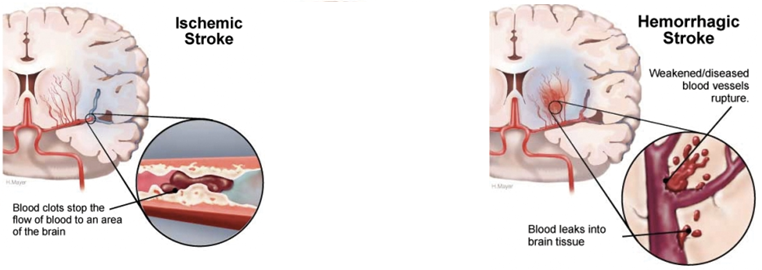
\includegraphics[scale=0.8]{figures/bProblemanalyse/haemoragisk_og_iskaemisk.png}
	\caption{På billedet ses, hvad der sker i hjernen, når henholdsvis iskæmisk og hæmoragisk apoplekså opstår. Der ses til venstre, at iskæmisk apopleksi sker, hvis en hjerneartierie blokkes. Til højre ses, at hæmoragisk apopleksi opstår, når en hjernearterie brister. [3]}
	\label{haem-isk}
\end{figure}

\subsection{Iskæmisk apopleksi}
Iskæmisk apopleksi opstår i 80-85\% af tilfældende iblandt det samlede antal af apopleksi ramte.[2] Her blokeres en hjernearterie af en blodprop, der stopper tilførslen af blod til et bestemt område i hjernen, hvilket ses på \figref{haem-isk}. Infarkterne dannes primært pga. åreforkalkning enten ved en trombe, der dannes på stedet, eller emboli fra hjertet.[5] Emboli består typsik af fragmenter af blodceller eller kolesterol, som er diffunderet ind i blodcirkulationen af hjernen fra en arterierne.[8] Derfor kan en hjertesygdom også være medvirkende til, at der opstår iskæmisk apopleksi, som f.eks. et hjerteanfald. En alvorlig blødning et andet sted på kroppen kan også resultere i blokeret eller stoppet blodtilførsel til hjernen.[7] Nervecellerne skades grundet iltmangel efter få minutter, og hvis dette fortsætter i en periode, vil de til sidst gå tabt. [5] % Specificer denne periode - hvor lang tid går der, før nervecellen går tabt?

\subsection{Hæmoragisk apopleksi}
Hæmoragisk apopleksi opstår i 10-15\% af tilfældende iblandt det samlede antal af apopleksi ramte.[2] Årsagen heraf skyldes hovedsageligt forhøjet blodtryk eller, i sjældnere tilfælde, bristede svagheder på arterier(aneurisme) eller medfødte misdannede kar.[5] Hæmoragisk apopleksi opstår, når en hjernearterie brister og lækage af blod danner en blodansamling, der beskadiger det omkringliggende væv og forøger trykket i hjernen, hvilket ses på \figref{haem-isk}. Blødning i selve hjernen(intracerebral hæmoragi) kommer af forhøjet blodtryk, der danner et pres på de små arterier, som får dem til at briste. [4] \\
Blødning i subaraknoidalrummet skyldes bristning af et aneurisme på en pulsåre i hjernen.[5] Symptomerne ved subaraknoidalblødning er generel tab af hjernefunktion, da der forekommer et øget pres på hjerneskallen, hvorimod ved intracerebral hæmoragi er hæmatomet lokaliseret et bestemt sted i hjernen og forårsager nedsat funktion ved én bestemt hjernefunktion[4]. 


%%%%%%%%%%%%%%%%%%%%%%%%%%%%%%%%%%%%%%%%%%%%%%%%%%%%                KILDER                 %%%%%%%%%%%%%%%%%%%%%%%%%%%%%%%%%%%%%%%%%%%%%%%%%%%%%%
% [1] = https://sundhedsstyrelsen.dk/da/udgivelser/2010/~/media/1A28F73140B54143B490B89DD687E3C9.ashx
% [2]: https://www.sundhed.dk/sundhedsfaglig/laegehaandbogen/hjerte-kar/tilstande-og-sygdomme/apopleksi-og-tia/apopleksi-og-tia-tci/#1 
% [3]: http://heart.arizona.edu/heart-health/preventing-stroke/lowering-risks-stroke 
% [4]: http://site.ebrary.com/lib/aalborguniv/reader.action?docID=10130864 (søgeord: hemorrage apoplexy)
% [5]: basisbog i sygdomslære: https://books.google.dk/books?id=vNK8CRu4t9sC&pg=PA444&lpg=PA444&dq=karokklusion&source=bl&ots=jAu__8N4Oz&sig=I4LKVLfRFQVE4NZYjHpUepM6jms&hl=da&sa=X&ved=0CEMQ6AEwB2oVChMI1Lbp_fv4xwIVCANzCh0AmgAV#v=onepage&q=apopleksi&f=false 
% [6]: Britannica - http://academic.eb.com.zorac.aub.aau.dk/EBchecked/topic/569347/stroke
% [7]: Hjernesagen - http://www.hjernesagen.dk/om-hjerneskader/bloedning-eller-blodprop-i-hjernen/fakta-om-apopleksi]
% [8]: Britannica - http://academic.eb.com.zorac.aub.aau.dk/EBchecked/topic/1800831/nervous-system-disease/75792/Stroke?anchor=ref606262




%%%%%%%%%%%%%%%%%%%%%%%%%%%%%%%%%%%%%%%%%%%%%%%%%%%%%%%%%%%%%%%%% Gamle ting
%Apopleksi er af World Health Organization (WHO) defineret som pludseligt opstået fokale neurologiske symptomer pga. forstyrrelser i hjernens blodcirkulation, der varer mere end 24 timer eller fører til døden[1gammel].
% [1gammel] = (Experience from a multicentre stroke register: a preliminary report.): http://www.ncbi.nlm.nih.gov/pubmed?cmd=Search&term=Bull%20WHO%20%5Bta%5D%20AND%2054%5Bvol%5D%20AND%20541%5Bpage%5D 